\documentclass{hw}
\title{Programming Assignment 1:\\ Implementing Lexical Analysis}

\usepackage{fancyvrb}
\usepackage{pervasives}
\usepackage{tikz}

\begin{document}
\maketitle

\section{Metadata}\label{sec:metadata}
% The fully qualified class name of your main program and any other
% instructions needed to run the program.
\begin{center}
\begin{BVerbatim}
make src
./xic --lex <xi_file.xi>...
\end{BVerbatim}
\end{center}

Our main executable is implemented in \texttt{mjw297.Main.java} which is found
in the \texttt{src/mjw297} directory. To build our executable, simply run
\texttt{make src}. Our Makefile depends only on \texttt{javac}; all our
dependencies are packaged in the \texttt{lib} directory, and we don't depend on
any external dependencies. Invoking \texttt{mjw297.Main} can be tricky because
you have to include the JARs inside of \texttt{lib} in your classpath. To run
our lexer, we recommend you use the \texttt{xic} script which invokes
\texttt{mjw297.Main} with everything configured properly. Note that we enabled
warnings when compiling with \texttt{javac}; also note that the lexing code
generated by JFlex and the Symbol class (used to represent tokens) generated by
CUP both generate warnings. These warnings will be seen when building our code.
To our knowledge, none of our own code generates warnings.

\section{Summary}\label{sec:summary}
In this programming assignment, we implemented a lexer in Java for the Xi
programming language using the JFlex lexer generator and CUP parser generator.
Our major design decisions involve the design of symbol and exception classes,
the choice of language and libraries, and the lexing of a few nefarious Xi
programs. The most challenging aspect of the assignment was the handling of
non-printable characters inside of comments, strings, and characters. For
example, the form feed character `\verb$\f$' is a non-printable character that
is difficult to lex correctly in various contexts. There are no known problems
with our implementation.

\section{Specification}\label{sec:specification}
In this section we make explicit our interpretation of the Xi language
specification and discuss various extensions to it which we have implemented.

\subsection{Line Endings and Whitespace}
The Xi language specification is ambiguous about the definition of a newline
referring to it only informally as a ``newline''. We define a line terminator
to be a carriage return `\verb$\r$', a newline `\verb$\n$', or both
`\verb$\r\n$'. If a `\verb$\r\n$' is present, it is counted as a single
newline. This definition of line terminators is consistent with the Java
Language
Specification\footnote{\url{https://docs.oracle.com/javase/specs/jls/se8/html/jls-3.html\#jls-3.4}}.
Similarly we define whitespace to be any of `\verb$\r$', `\verb$\n$',
`\verb$\r\n$', `\verb$ $', `\verb$\t$', `\verb$\f$'. This also consistent with
the Java Language
Specification\footnote{\url{https://docs.oracle.com/javase/specs/jls/se8/html/jls-3.html\#jls-3.6}}.

\subsection{Comments}
The Xi language specification states that a comment is \texttt{//} followed by
any sequence of characters until a newline character. We interpret a newline
character to be any line terminator as defined above. We have also made a small
revision and allow comments to be terminated by the end of a file in addition
to a line terminator. This rule avoids the rather counter-intuitive scenario
where a file ends in a comment and leads to a lexing error.

\subsection{Characters in Comments, Strings, and Characters}
Xi input files are UTF-8 encoded, though keywords and identifiers are made up
of only ASCII characters. This leads to the question of what characters are
allowed inside of comments, strings, and character literals. We allow any
character that is not a line terminator, including exotic Unicode characters,
to appear in a comment, string, or character literal. Allowing exotic
characters simplifies the lexer and is also flexible.

\subsection{Hex and Unicode Escape Sequences}
The programming assignment mandates that we support hex escape sequences inside
of string and character literals. For example, the string \verb$"\x64"$ is
lexed into the string \texttt{"d"}. The programming assignment is ambiguous
about the format of the hex escape sequences. We support only fixed width
two-digit hex escape sequences.
%
In addition to hex escape sequences, we have also added Unicode escape
sequences of the form:
\begin{center}
  \verb$\u[a-fA-F0-9][a-fA-F0-9][a-fA-F0-9][a-fA-F0-9]$
\end{center}
For example, the string \verb$"\u0064"$ lexes to \texttt{"d"}.

\subsection{Escape Characters}
The Xi language specification says to support a ``reasonable'' set of character
escapes. We have elected to support \verb$\t$, \verb$\b$, \verb$\n$, \verb$\r$,
\verb$\f$, \verb$\'$, \verb$\"$, and \verb$\\$. These are also the set of
non-printable characters that our lexer pretty prints. For example the Xi
string \verb$"\n"$ is printed as \verb$\n$. All other non-printable
characters are printed as hex escaped sequences.

\subsection{Non-Line Terminating Whitespace}
Certain whitespace character are not Xi line terminators but are often
considered in other contexts to be line terminators. For example, \verb$\f$,
\verb$\u2028$, and \verb$\u2029$ are considered by JFlex to be line
terminators.  This leads to an inconsistency in the row numbers our lexer
reports. The number of lines reported by JFlex is not consistent with the
number of lines terminated by a Xi line terminator. Since these whitespace
characters are rare to see in source code and since the inconsistency is
unimportant, we avoid the complexity of correcting this inconsistency.

\section{Design and Implementation}\label{sec:design}
\subsection{Architecture}
\begin{center}
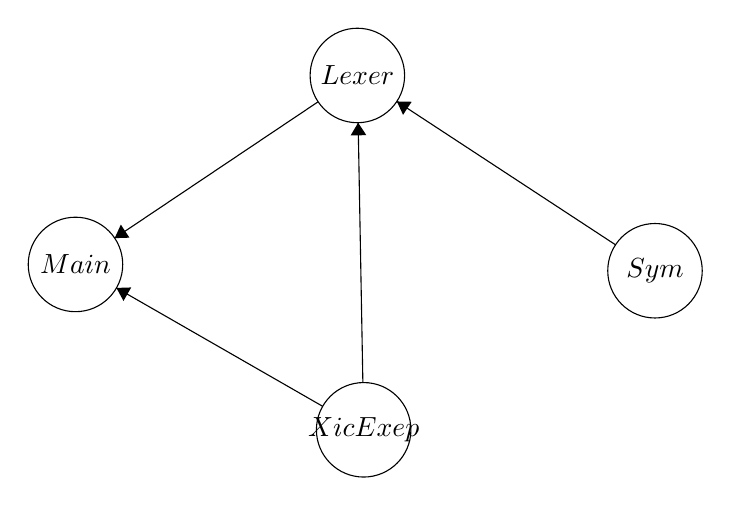
\begin{tikzpicture}[scale=0.2]
\tikzstyle{every node}+=[inner sep=0pt]
\draw [black] (36.8,-14.9) circle (3);
\draw (36.8,-14.9) node {$Lexer$};
\draw [black] (37.2,-37.4) circle (3);
\draw (37.2,-37.4) node {$XicExep$};
\draw [black] (55.7,-27.3) circle (3);
\draw (55.7,-27.3) node {$Sym$};
\draw [black] (18.9,-26.9) circle (3);
\draw (18.9,-26.9) node {$Main$};
\draw [black] (34.31,-16.57) -- (21.39,-25.23);
\fill [black] (21.39,-25.23) -- (22.33,-25.2) -- (21.78,-24.37);
\draw [black] (37.15,-34.4) -- (36.85,-17.9);
\fill [black] (36.85,-17.9) -- (36.37,-18.71) -- (37.37,-18.69);
\draw [black] (53.19,-25.65) -- (39.31,-16.55);
\fill [black] (39.31,-16.55) -- (39.7,-17.4) -- (40.25,-16.57);
\draw [black] (34.6,-35.91) -- (21.5,-28.39);
\fill [black] (21.5,-28.39) -- (21.95,-29.22) -- (22.44,-28.36);
\end{tikzpicture}
\end{center}

We had four main classes in our lexer:
\begin{enumerate}
  \item{Main:} This is the main front end for our compiler. In this class, we
  handle the various command line options passed into the binary and call the
  rest of our lexing code. We also handle all IO (including the lexing analysis
  output) in this class.

  \item{Lexer:} This class is generated by JFlex from our lexer specification.
  It is used to tokenize source Xi files.

  \item{Symbol:} This class, generated by CUP, is our main internal representation
  of tokens.

  \item{XicException:} We subclass this abstract class to throw lexing errors (e.g.
  empty characters) which we then handle internally.
\end{enumerate}
\subsection{Code Design}
One of the main extensions we implemented was in comments. The project spec specified that
comments were only to be terminated by a newline, but we allowed comments that were
terminated by any line terminals (\verb$\r$, \verb$\r\n$, and \verb$\n$) and by EOF.
We added the EOF case since it is conceivable that programmers would end a source file
with a comment, and having a lexing failure in this case would be undesireable. 

% TODO: BigNum %

We also added extensive lexical error support by way of our XicException class. While
the examples only gave the empty character exception, we added several other error cases,
such as out of bounds long literals, invalid hex literals, unterminated strings and
character literals, and invalid tokens (a catch all for symbols unsupported in the
language specification).

\subsection{Programming}
We implemented our lexer using both a bottom-up and a top-down approach. Some
members of our team used a bottom-up approach to implement our
\texttt{XicException} exception class and \texttt{Symbol} symbol class---both
of which do not depend on any other class---without knowing exactly how they
would be used by other classes. Conversely, other members implemented our
\texttt{Main} class without yet knowing the specific implementation of the
underlying lexer implementation. We also followed the designed principle of
test driven development, implementing tests cases as we implemented our lexer
to catch bugs often and early. This is described in detail in \secref{testing}.

We encountered various issues while implementing our lexer, most of which
revolved around the subtle interactions between whitespace characters and
regular expressions that are more complicated than they seem. The most
obnoxious issue revolved around the following regular expression we initially
used to match comments.

\begin{center}
\begin{BVerbatim}
LineTerminator = \n | \r | \r\n
Comment = "//" (!{LineTerminator})* {LineTerminator}
\end{BVerbatim}
\end{center}

Intuitively, the \texttt{Comment} regular expression matches \texttt{//}, any
number of characters that aren't \verb$\r$, \verb$\n$, or \verb$\r\n$, and
finally a line terminator. Surprisingly though, the string \verb$//a\r\na\n$ is
lexed as a single comment, not as a comment and then an identifier \verb$a$!
Inspecting the regular expression deeper, we see the language of
\verb${Comment}$ is \verb${\r, \n, \r\n}$. The language of \verb$!{Comment}$ is
then everything that's not in \verb${\r, \n, \r\n}$. This set includes
\verb$a\r$ and \verb$\na$! Thus, \verb$a\r\na$ is matched by
\verb$(!{LineTerminator})*$.

The distribution of work is described in detail in \secref{workplan}.

\section{Testing}\label{sec:testing}
We wrote JUnit tests to test our lexer. We started with very basic tests that
would test one token at a time. Then we moved on to more complex tests where
we would mix up different tokens or add random white spaces before, after or between the
tokens. After that we created more test cases with escape characters, line terminators
and EOF. Lastly, we created invalid tests to make sure that we are throwing the correct
exceptions.

Our test plan worked out very well. First testing on very basic tokens helped us solidify
the majority of our code. Then, testing with escape characters and line terminators helped
us find a lot of bugs in our code and made sure that we were dealing with white spaces correctly.
Finally, testing that exceptions were thrown properly again made sure we covered all the corner
cases in our lexer.
\section{Work Plan}\label{sec:workplan}
Before we started coding one person set up the skeleton code and modularization. Then another
member took care of the frontend such as command line interfaces. Then other people
wrote the rules for lexing while the other members wrote test cases.
\section{Known Problems}\label{sec:problems}
None.
\section{Comments}\label{sec:comments}
We spent about 60 hours total on the assignment. The assignement overall introduced
important concepts about lexing but we thought the coding was a little bit dry and tedious.
\end{document}
